\section{Related Work}
\begin{figure}[t]
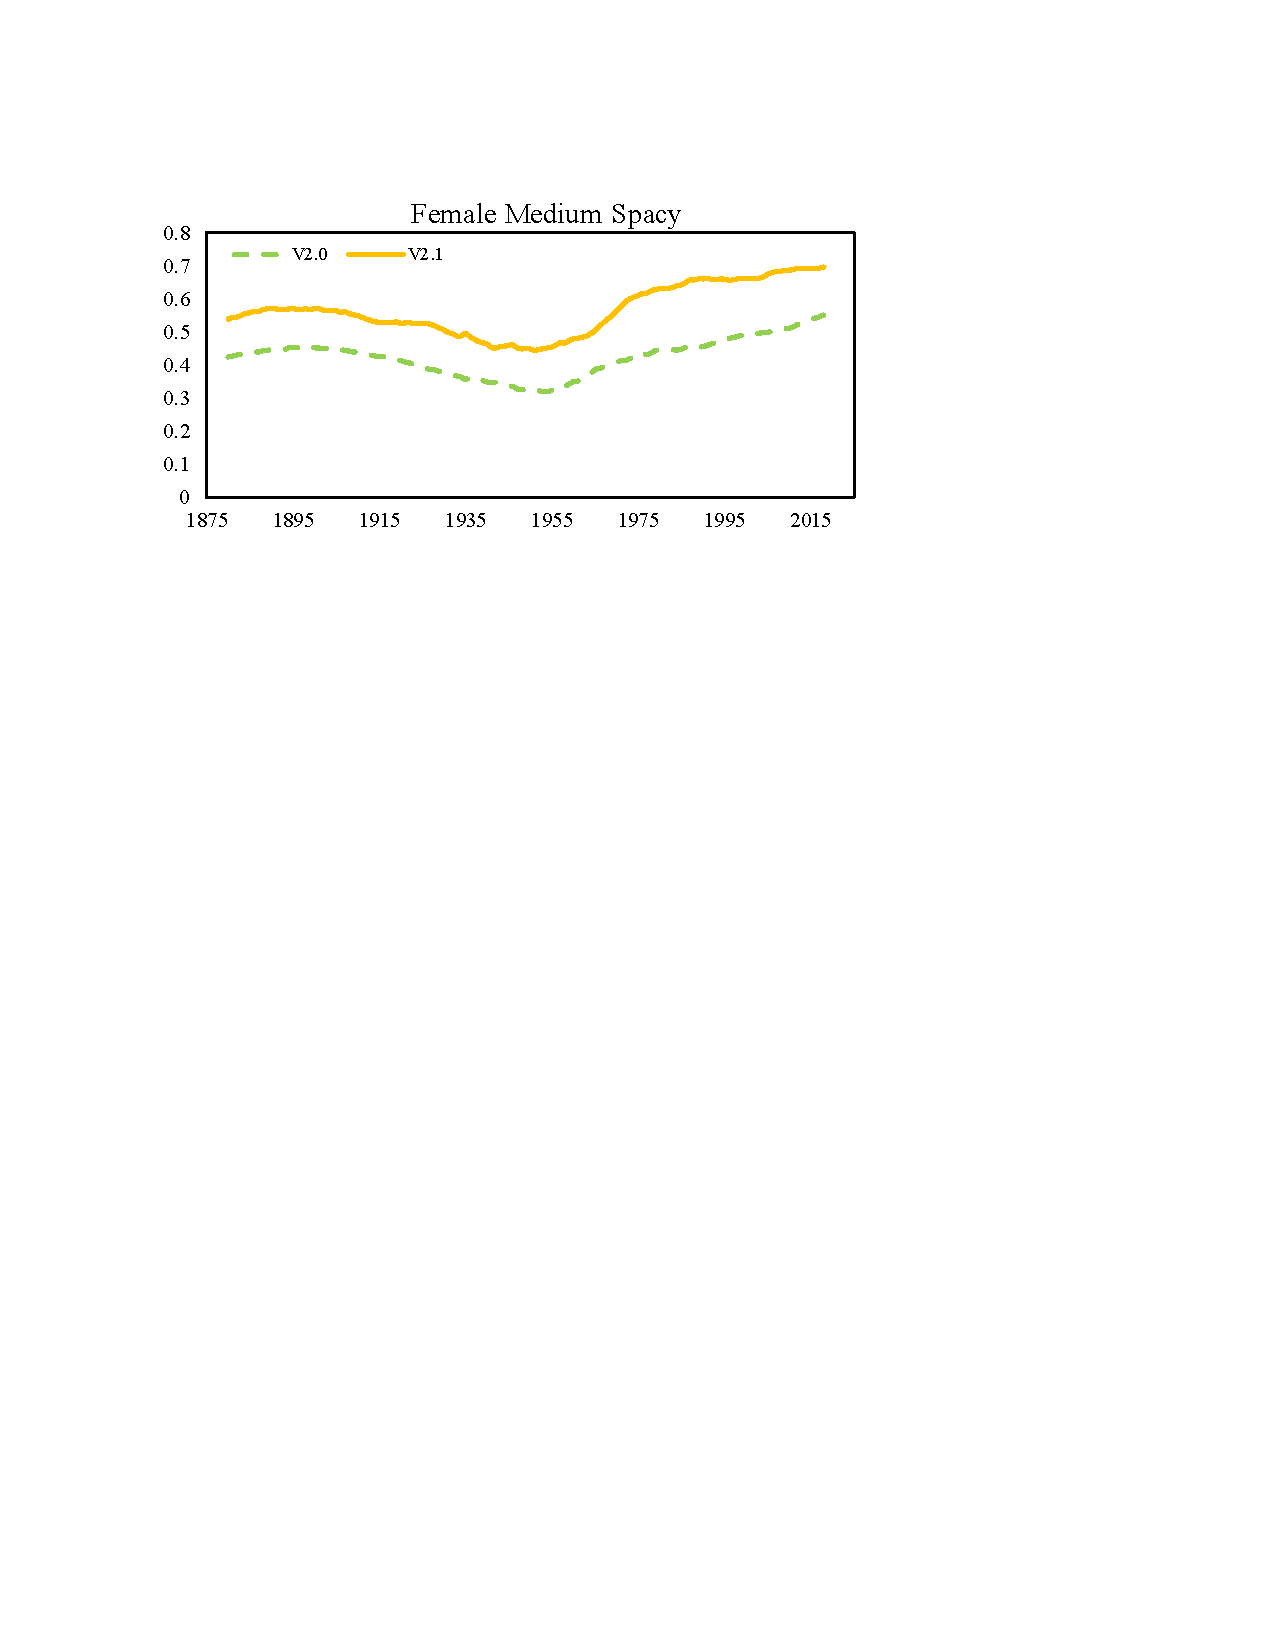
\includegraphics[width=0.45\textwidth,height=0.2\textwidth,trim=0cm 0cm 0cm 0cm,clip=true]{images/version_results/version_results_female.pdf}
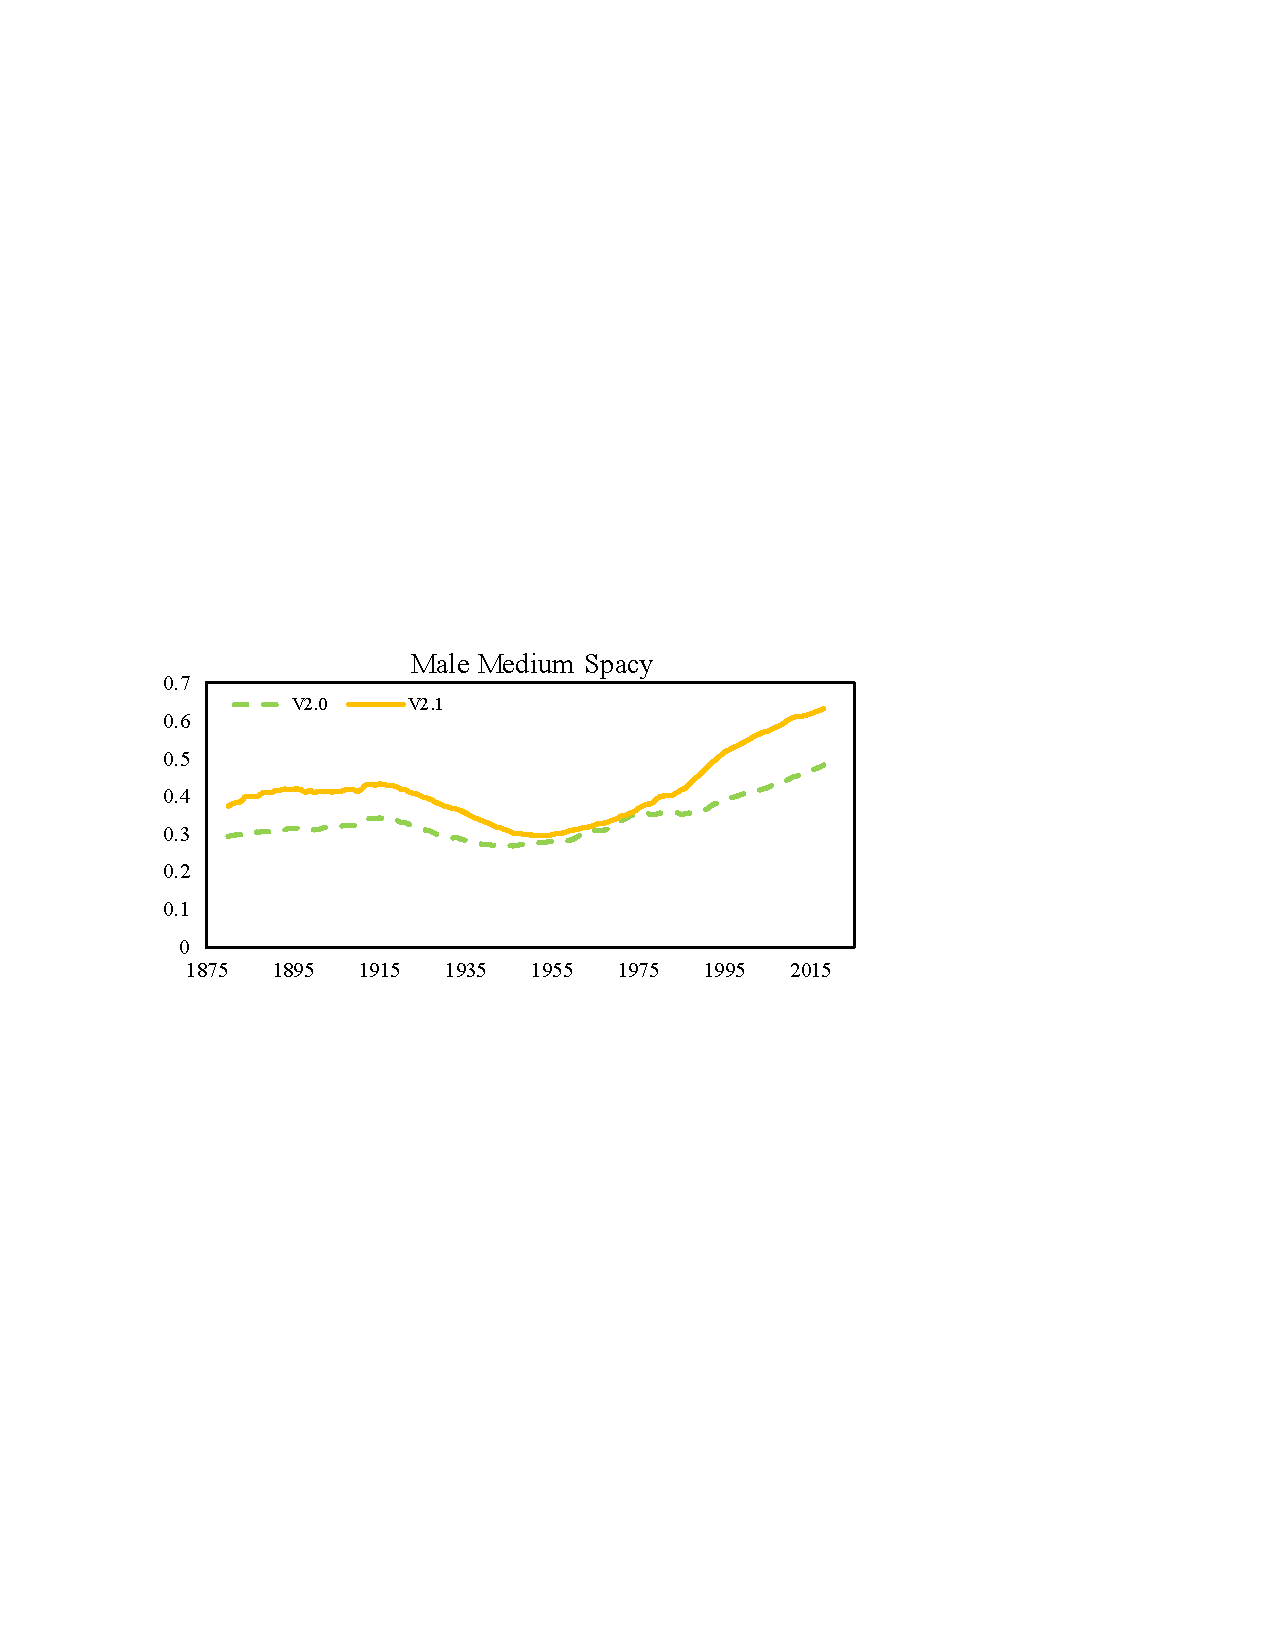
\includegraphics[width=0.45\textwidth,height=0.2\textwidth,trim=0cm 0cm 0cm 0cm,clip=true]{images/version_results/version_results_male.pdf}
\caption{Biased performance of version 2.1 over 2.0 in Spacy medium. The bias against female names was on average twice that of male names.}
\label{spacyv}
\end{figure}
We have seen large amounts of attention and work regarding fairness in machine learning and natural language processing models and methods. Recent papers observed a type of stereotyping bias in word embedding methods and tried to mitigate this type of bias by proposing a method that respects the embeddings for gender-specific words but de-biases embeddings for gender-neutral words \cite{bolukbasi2016man}, or by generating a gender-neutral version of Glove (called GN-Glove) that aims to preserve gender information in some directions of word vectors, while setting other dimensions free from gender influence \cite{zhao2018learning} or other data augmentation techniques \cite{pmlr-v97-brunet19a,zhao2019gender}. Other work tried to show and address bias in co-reference resolution \cite{zhao2018gender}, semantic role labeling \cite{zhao2017men}, machine translation \cite{font2019equalizing}, language models \cite{bordia2019identifying}, and sentence embedding \cite{may2019measuring}.

Addressing fairness and bias, not only in NLP but also in general machine learning, has lately gained much attention. 
\begin{table}
%\centering
\begin{tabular}{ p{1.2cm} p{3.3cm} p{3.2cm}}
 \toprule
 Female Name&CoreNLP version 3.8&CoreNLP version 3.9\\
 \midrule
 Isabel&Not Tagged&Tagged as MISC\\[0.5pt]
 Angelina&Not Tagged&Tagged as MISC\\[0.5pt]
 June&Not Tagged&Tagged as DATE\\[0.5pt]
 Charlotte&Tagged as LOCATION&Tagged as CITY\\[0.5pt]
 Victoria&Tagged as LOCATION&Tagged as CITY\\[0.5pt]
 Sydney&Tagged as LOCATION&Tagged as CITY\\[0.5pt]
  \bottomrule
\end{tabular}
\newline
\vspace*{0.3 cm}
\newline
\begin{tabular}{ p{1.2cm} p{3.3cm} p{3.2cm}}
 \toprule
 Male Name&CoreNLP version 3.8&CoreNLP version 3.9\\
 \midrule
 Christian&Not Tagged&Tagged as RELIGION\\[0.5pt]
 Logan&Tagged as LOCATION&Tagged as CITY\\[0.5pt]
 Roman&Not Tagged&Tagged as MISC\\[0.5pt]
 Santiago&Tagged as LOCATION&Tagged as CITY\\[0.5pt]
 Jordan&Tagged as LOCATION&Tagged as CITY\\[0.5pt]
 Messiah&Not Tagged&Tagged as TITLE\\[0.5pt]
 \bottomrule
\end{tabular}
\caption{Some examples on how tagging changed during version update of the CoreNLP model. Note how the original problem of tagging PERSON entities correctly has not been addressed.}
    \label{corenlp_version_examples}
\end{table}
In \citet{mehrabi2019survey}, the authors created a taxonomy on fairness and bias that discusses how researchers have addressed fairness related issues in different fields. From representation learning \cite{moyer2018invariant} to graph embedding \cite{bose2019compositional} to community detection \cite{mehrabi2019debiasing} and clustering \cite{pmlr-v97-backurs19a}, researchers have studied biases in these areas and tried to address them by pointing out the observed problems and proposing new directions and ideas. In \citet{buolamwini2018gender} authors show and analyze the existing gender bias in facial recognition systems, such as those used by IBM, Microsoft, and Face++, and created a benchmark for better evaluation of bias in facial recognition systems. This is considered a significant contribution as it opens many future research questions and related papers. Paying attention to different AI applications and pointing out their issues in terms of fairness is an important issue that needs serious attention for significant future improvements to these systems. 




%Bias in machine learning and NLP is an important issue that needs consideration and more attention as these models play an important role in our lives and we want our models to be away from any human like stereotyping or bias. Being observant and noticing problems that can affect these models is really important and a major step toward mitigating issues related to fairness. 
